\documentclass[12pt]{article}

\usepackage[portuguese]{babel}
\usepackage{graphicx}
\usepackage[section]{placeins}
\usepackage{float}
\usepackage{url}

\graphicspath{ {figures} }

\author{Rafael Begnini de Castilhos}
\title{Segundo trabalho prático (Wireshark e SNMP)}
\date{\today}

\addto\captionsportuguese{\renewcommand*\contentsname{Sumário}}

\begin{document}

\maketitle

\begin{abstract}
O presente relatório possui como objetivo demonstrar a utilização e gerenciamento de rede com as ferramentas o PRTG e o Wireshark, com o fito de prover ao leitor a base necessária para entendimento  do uso desses \emph{softwares} e replicar os experimentos realizados. Fazendo o uso dos programas foi realizado um monitoramento de aproximadamente 3 horas por dia num período de 4 dias. Durante o monitoramento foram compreendidos conceitos importantes sobre os protocolos utilizados como \emph{ARP} e \emph{SNMP}. Proporcionando um melhor entendimento de como gerenciar uma rede doméstica, verificando a eficiência da mesma.
\end{abstract}

\tableofcontents

\section{Introdução}

Nesse relatório será demonstrado o trabalho prático realizado utilizando as ferramentas PRTG e Wireshark. Desse modo será possível realizar um monitoramento para ajudar a compreender o tráfego de pacotes entre os dispositivos de uma rede doméstica. As ferramentas utilizadas são de alta credibilidade e sucesso no mercado da tecnologia da informação, com isso, o compreendimento da utilização delas é imprescindível para um profissional da computação que deseje trabalhar com o gerenciamento de redes de computadores.

\section{Ferramentas de gerência}

\subsection{PRTG}

O PRTG Network Monitor é uma ferramenta de monitoramento de rede. A instalação é feita em um computador centralizador e os outros dispositivos da rede não necessitam de qualquer instalação ou configuração. Além do mais, o software conta com uma interface web prática, eficiente e com excelente usabilidade, permitindo gerar relatórios, gráficos e visualizações automaticamente, de acordo com as métricas extraídas. Entretanto, o software é restrito à plataforma Windows, além de que por se tratar de um software proprietário com um \emph{trial} de 30 dias o acesos a ele é mais restrito do que a suas alternativas \emph{open-source}.

\subsection{Wireshark}

O Wireshark é uma ferramenta para monitoramento de pacotes que permite verificar a entrada e saída de dados do computador, sendo \emph{open-source} e gratuita . Diferentemente do PRTG, possui suporte para diversas plataformas e todos os recursos estão disponíveis gratuitamente.

\section{Topologia da rede}

O monitoramento foi executado em uma rede doméstica, utilizando os serviços da AdylNet Telecom, tendo conectados nas redes os seguintes dispositivos: Um notebook Lenovo Thinkpad, um notebook Acer AspireF5, um desktop customizado e um Raspberry PI Zero W. O PRTG foi instalado no notebook Lenovo Thinkpad, devido a maior robustez dessa máquina, os outros dispositivos foram adicionados ao monitoramento pelo painel do PRTG, com sensores de Ping e SSH estabelecidos. Todos os dispositivos foram utilizados posteriormente na análise do Wireshark.

\begin{figure}[H]
    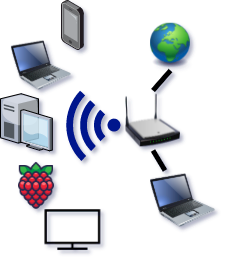
\includegraphics{topologia.png}
    \caption{Um notebook Lenovo Thinkpad (192.168.0.151) conectado com fio ao roteador, um notebook Acer AspireF5 (192.168.0.101), um desktop (192.168.0.80), um Raspberry PI Zero W (192.168.0.38), um Smartphone Motorola X4 (192.168.0.220), uma TV Samsung Smart e um Modem com roteador (192.168.0.1)}
\end{figure}

\subsection{Equipamentos}

\begin{itemize}
    \item Desktop  (192.168.0.80)
    \begin{itemize}
        \item Processador: Intel i7 3770 6.30 GHz
        \item Memória RAM: 16GB DDR4 3000Mhz
        \item Placa de vídeo: NVIDIA GeForce GTX 660
        \item Sistema Operacional: Ubuntu 20.04
        \item Adaptador Ethernet: Realtek PCIe
    \end{itemize}
    \item Notebook Lenovo Thinkpad (192.168.0.151)
    \begin{itemize}
        \item Processador: Intel i7 8565U 4.60 GHz
        \item Memória RAM: 16GB DDR4 3000Mhz
        \item Placa de vídeo: Intel UHD 620
        \item Sistema Operacional: Windows 10
    \end{itemize}
    \item Notebook Acer AspireF5 (192.168.0.101)
    \begin{itemize}
        \item Processador: Intel i5 7200U 2.50 GHz
        \item Memória RAM: 8GB DDR4 3000Mhz
        \item Placa de vídeo: NVIDIA GeForce 940MX
        \item Sistema Operacional: Mint Uma 20.2
        \item Adaptador Ethernet: Realtek PCIe
    \end{itemize}
    \item RaspberryPI Zero W (192.168.0.38)
    \begin{itemize}
        \item Processador: ARM v6 1.00 GHz
        \item Memória RAM: Memória 512MB
        \item Sistema Operacional: Raspberry Pi OS
    \end{itemize}
    \item Smartphone Motorola X4 (192.168.0.220)
    \begin{itemize}
        \item Sistema Operacional: Android 9
    \end{itemize}
    \item TV Samsung Smart
    \item Modem (192.168.0.1)
    \begin{itemize}
        \item Modelo: TP-Link WR740N
        \item Frequência: 2.4 GHz
    \end{itemize}
\end{itemize}

\section{Monitoramento}

O PRTG diferencia os dispositivos entre Sonda e Rede, sendo que o primeiro diz respeito a dispositivos que possuem o PRTG definido como agente centralizador, enquanto o segundo são os dispositivos conectados na rede e visualizados por meio de protocolos de rede apenas. Durante esse trabalho foi utilizado apenas uma Sonda devido a impossibilidade de instalar outros na rede, tendo em vista que o PRTG é instalável apenas no Windows e os outros computadores da rede utilizam Unix.

\subsection{Funcionamento da Sonda}

\begin{figure}[H]
    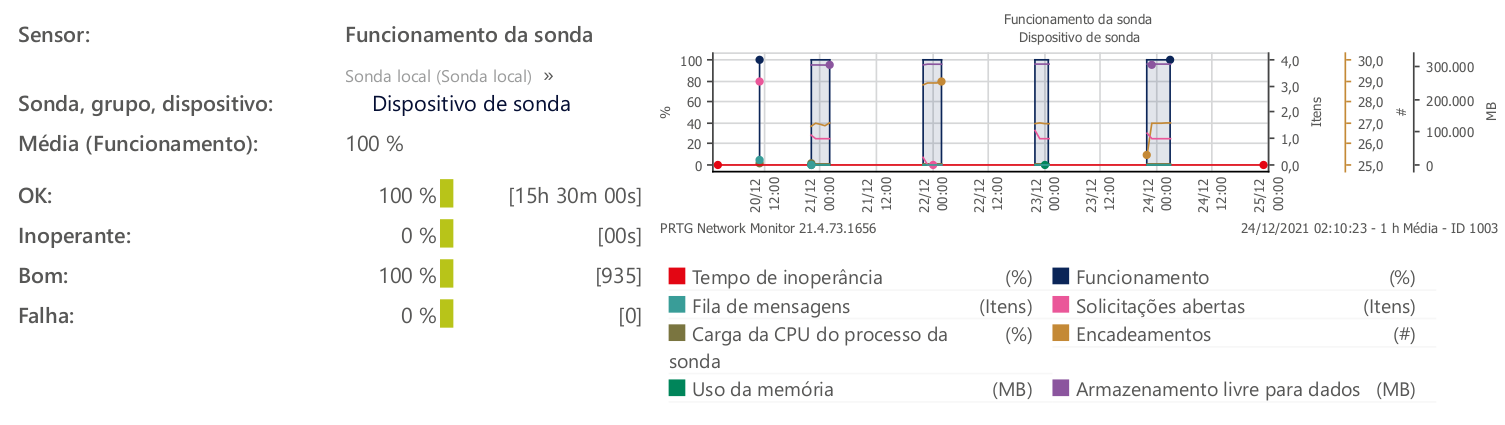
\includegraphics[width=\linewidth]{probe_health.png}
    \caption{Gráfico do sensor Probe Health gerado pelo PRTG.}
\end{figure}

O sensor de saúde da sonda demonstra com detalhes métricas de funcionamento da sonda em relação ao PRTG, como \emph{downtime}, uso de memória, número de \emph{threads} e \emph{CPU load}.

\subsection{Funcionamento do Sistema}

\begin{figure}[H]
    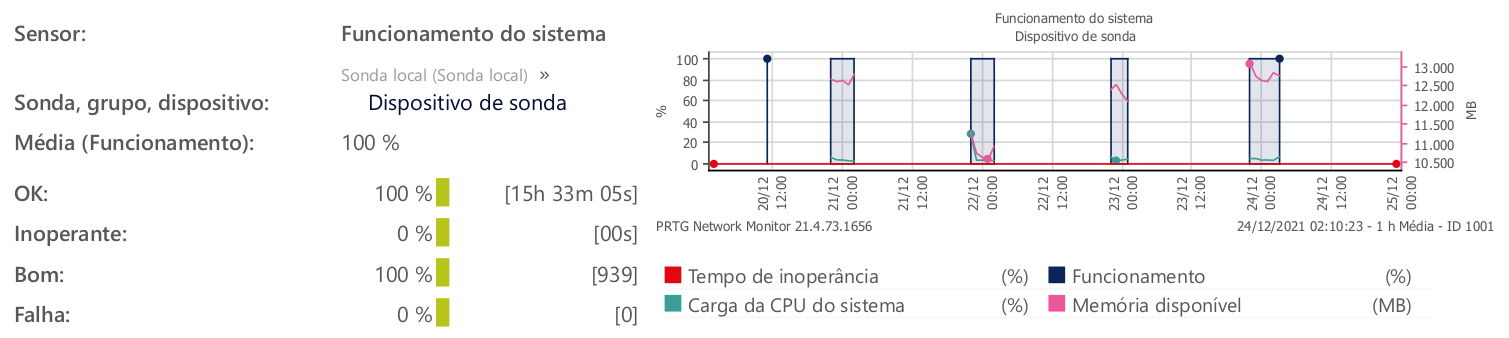
\includegraphics[width=\linewidth]{system_health.png}
    \caption{Gráfico do sensor System Health gerado pelo PRTG.}
\end{figure}

O sensor de saúde do sistema monitora o \emph{hardware} do sistema hospedeiro, a fim de verificar picos de uso do sistema e as causas deles.

\subsection{Funcionamento de Software como serviço}

\begin{figure}[H]
    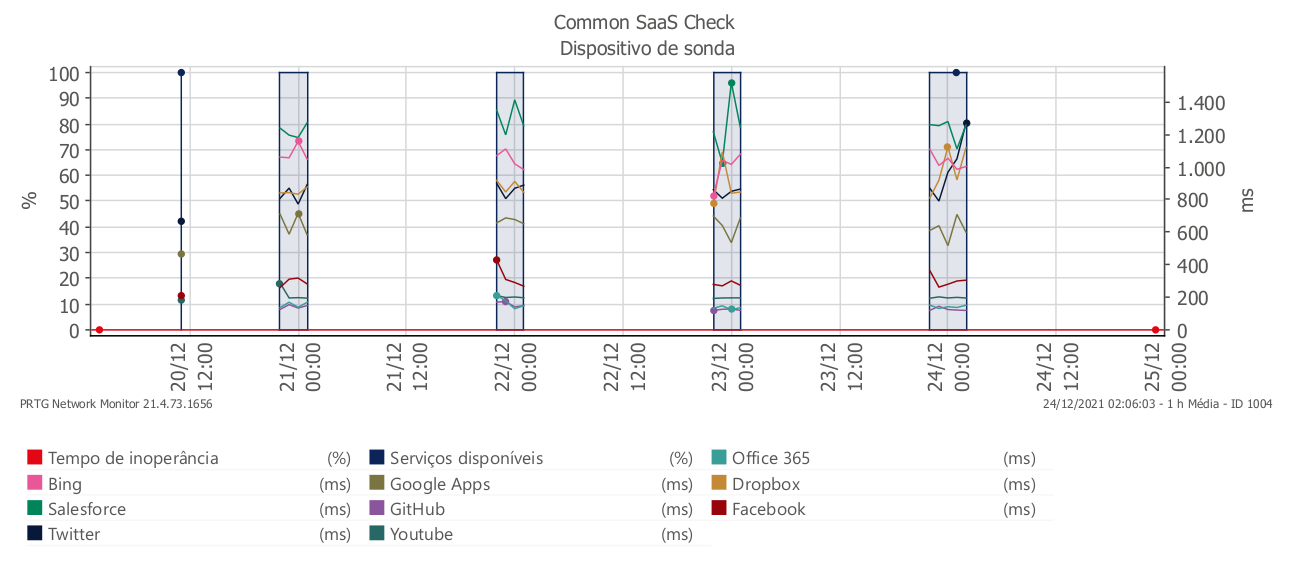
\includegraphics[width=\linewidth]{saas.png}
    \caption{Gráfico do sensor de funcionamento de Software como serviço gerado pelo PRTG.}
\end{figure}

A sonda Common SaaS Check verifica se os provedores estão disponíveis, são eles os principais: Bing, Twitter, Github, Youtube, Office 365, Dropbox e Facebook. Esse sensor verifica a disponibilidade (em forma de ping) de serviços online comuns a serem utilizados em um escritório, pode ser muito útil no gerenciamento de uma rede corporativa. Durante a maior parte dos serviços se manteve abaixo de 1000ms, mas podemos destacar um pico e média mais elevada no serviço da Salesforce.

\subsection{Ping}

\begin{figure}[H]
    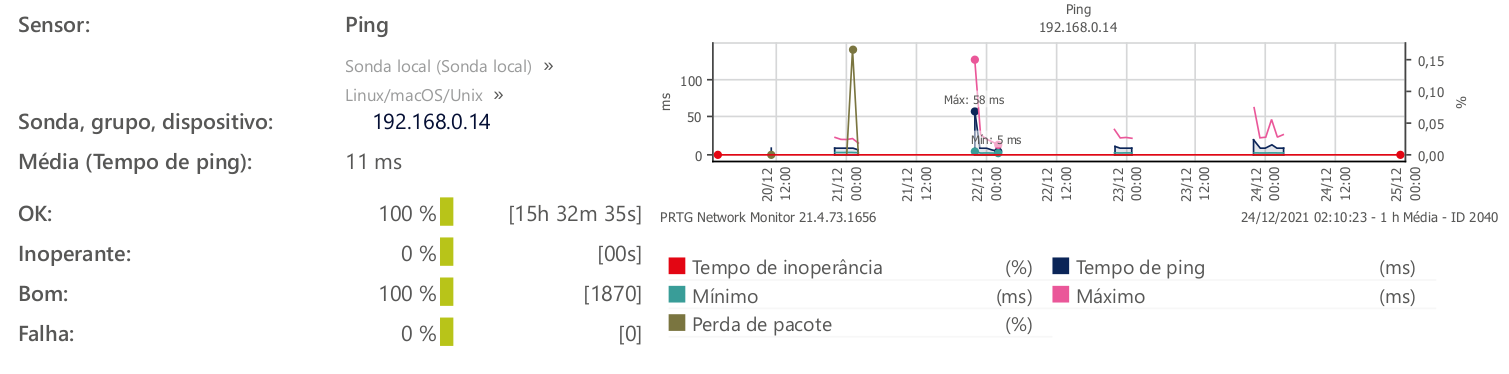
\includegraphics[width=\linewidth]{ping.png}
    \caption{Gráfico do sensor Ping gerado pelo PRTG.}
\end{figure}

O sensor de ping monitora o tempo de resposta um ping pelo protocolo TCP/IP, o PRTG permite monitorar pings para quaisquer dispostivos da rede, no monitoramento foi abaixo foram realizados pings para o Desktop citado na sessão de topologia de rede.

\subsection{Http}

\begin{figure}[H]
    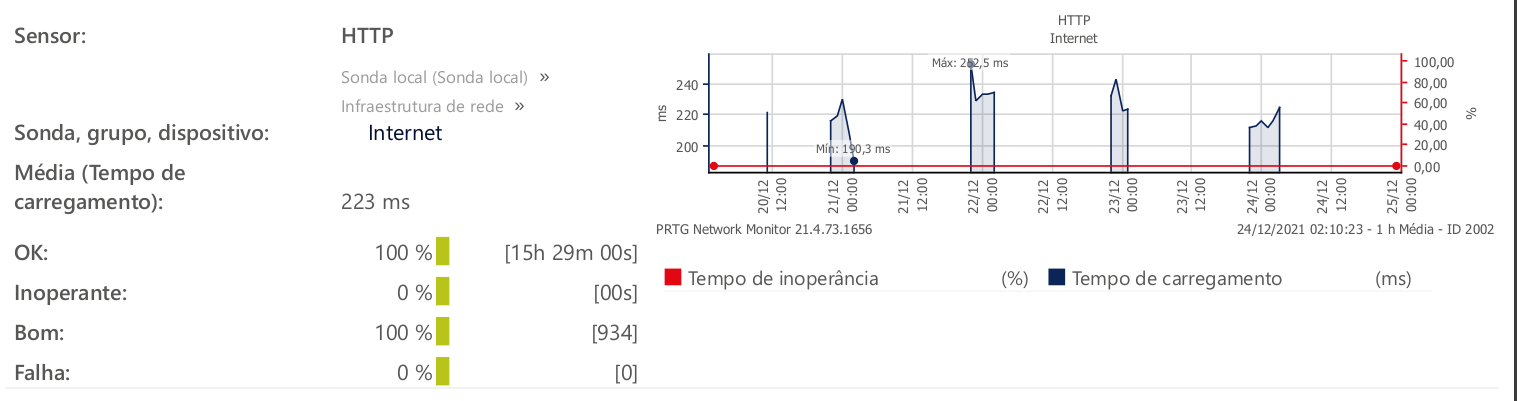
\includegraphics[width=\linewidth]{http.png}
    \caption{Gráfico do sensor Http gerado pelo PRTG.}
\end{figure}

O HTTP monitora o tempo de carregamento de uma página na internet. Nota-se que houve um pico anormal de 252.5 ms e um mínimo de 190.3 ms. Site utilizado no momento: www.google.com.

\section{Wireshark}

\subsection{Address Resolution Protocol (ARP)}

O Address Resolution Protocol (ARP) transforma endereços da camada da internet (normalmente um endereço IPV4) em endereços da camada de enlace (como por exemplo um endereço MAC), esse protocolo é essencial para o funcionamento da internet e de redes locais. No Wireshark podemos monitorar o funcionamento do protocolo ARP por meio de um filtro, já que o \emph{software} tem em sua configuração padrão a capacidade de monitorar o protocolo.

A imagem abaixo foi obtida após um monitoramento de 10 minutos contínuos no Wireshark, com o filtro \emph{arp} ligado (dessa forma o software ignora todos os outros protocolos e comunicações). É possível perceber que o dispositivo Desktop envia pela rede um pedido de identificação do dispositivo RaspberryPI Zero W. Também vemos uma troca de mensagens entre o Desktop e o roteador TPLink, quando o Desktop pergunta ao roteador qual seu endereço MAC.

\begin{figure}[H]
    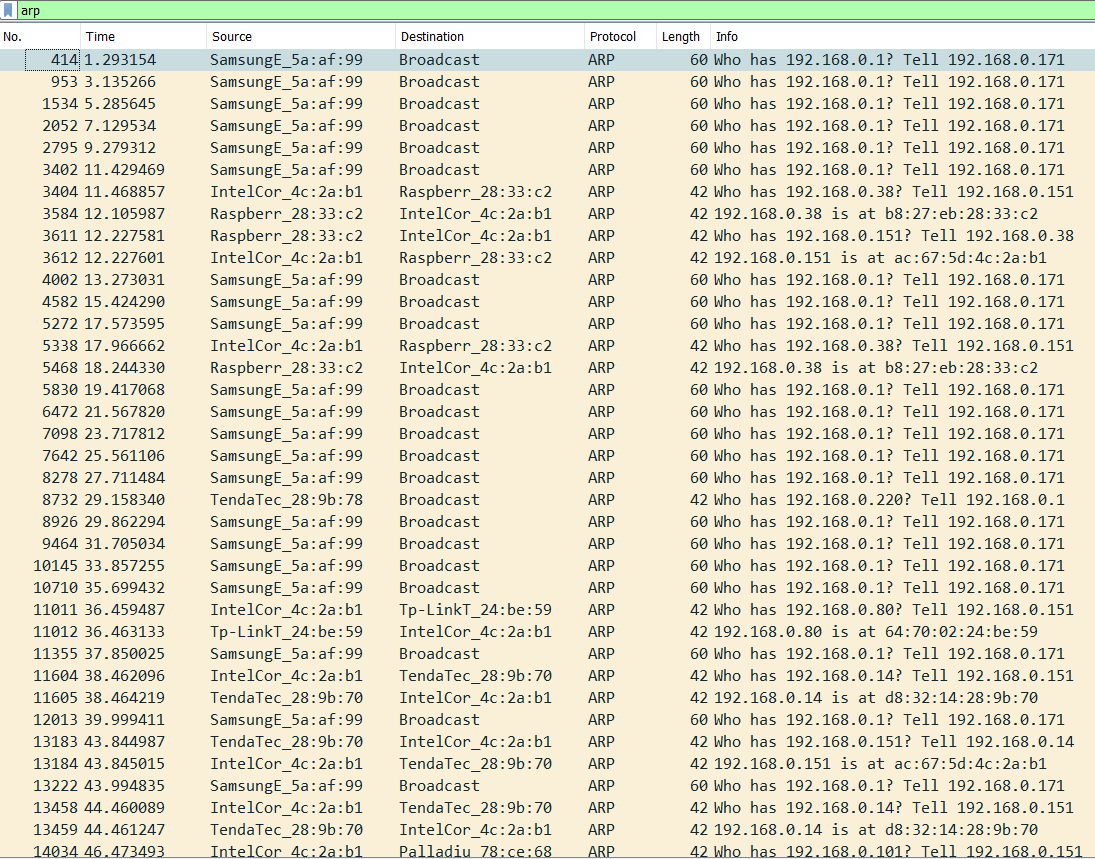
\includegraphics[width=\linewidth]{ARP.png}
    \caption{Tabela de ocorrências do protocolo ARP monitoradas pelo Wireshark.}
\end{figure}

\subsection{Simple Network Management Protocol (SNMP)}

Simple Network Management Protocol é um protocolo para organização de dispositivos gerenciados em uma rede IP, o Wireshark também é capaz de captar nativamente as trocas de mensagens relativas ao SNMP, por meio do filtro \emph{snmp} podemos configurar o software para mostrar apenas essas mensagens.

Na imagem abaixo foi realizado um monitoramento por duas horas com objetivo de capturar mensagens relativas ao SNMP. As transmissões interceptadas foram realizadas pelo dispositivo de IP 192.168.0.80 (Desktop), 192.168.0.151 (Notebook Lenovo Thinkpad) com o destino sendo a subrede 255.255.255.255. Outra transmissão em específico é a do dispositivo 192.168.0.101 (Notebook Acer AspireF5) que possui como destino (192.168.0.1) que é o modem roteador. Entretanto percebe-se o protocolo ICMP, que acontece quando o adaptador \emph{wireless} conectado ao notebook é removido propositalmente. 

\begin{figure}[H]
    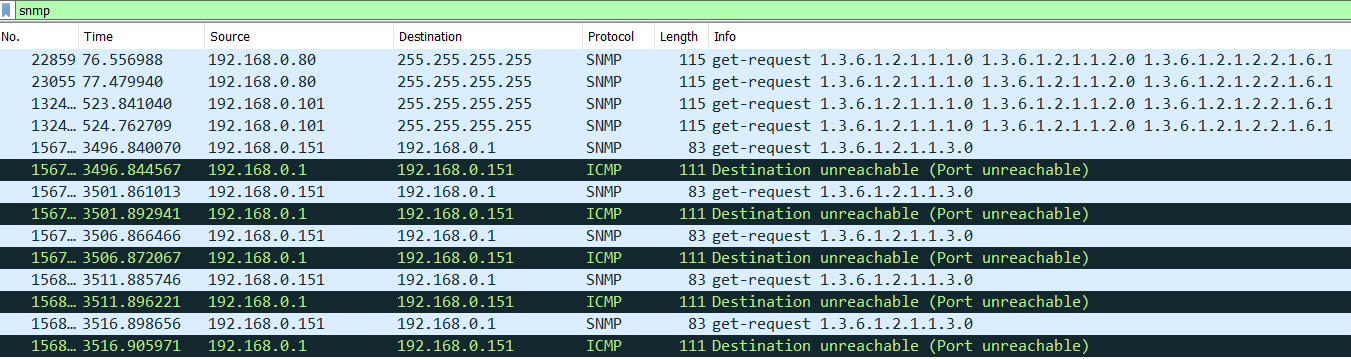
\includegraphics[width=\linewidth]{SNMP.png}
    \caption{Tabela de ocorrências do protocolo SNMP monitoradas pelo Wireshark.}
\end{figure}

\section{Conclusão}

Para realizar com sucesso os procedimentos foi necessário pesquisar e entender o funcionamento de ferramentas utilizadas na gerência de redes. Utilizando essas ferramentas e determinadas funcionalidades, foi possível denotar o funcionamento de uma rede doméstica e seus detalhes específicos, podendo utilizar esses conhecimentos para otimizar a rede e os processos envolvidos. Portanto, fica evidente a importância desse trabalho na agregação de conhecimento, visto que existem inúmeros aplicações perante a sociedade hodierna.

\nocite{*}
\medskip

\bibliographystyle{abbrv}
\bibliography{biblio}

\end{document}